\section{Design pattern}

\begin{frame}
    \frametitle{Refactoring with the strategy pattern}
    \textbf{Problem:} Methods for I/O and calculations will change frequently

    \textbf{Solution:} Strategy as the implemented design pattern

    \begin{columns}
        \hspace{-25pt}
        \begin{column}{0.55\textwidth}
            \begin{itemize}
                \item Define a family of algorithms and encapsulate them
                \item \textbf{Structure: } 
                \begin{itemize}
                    \item Simulation as the highest layer for choosing strategy
                    \item Compartmentalizing I/O, model and physics
                    \item Enabling Combinations of physics functions through strategy
                \end{itemize}
                \item \textbf{Benefits: }
                \begin{itemize}
                    \item Simple swapping of algorithms
                    \item Isolation of implementation details
                    \item Open/Closed Principle: Introduction of new strategies without context change
                \end{itemize}
            \end{itemize}
        \end{column}
        \begin{column}{0.45\textwidth}
            \begin{figure}
                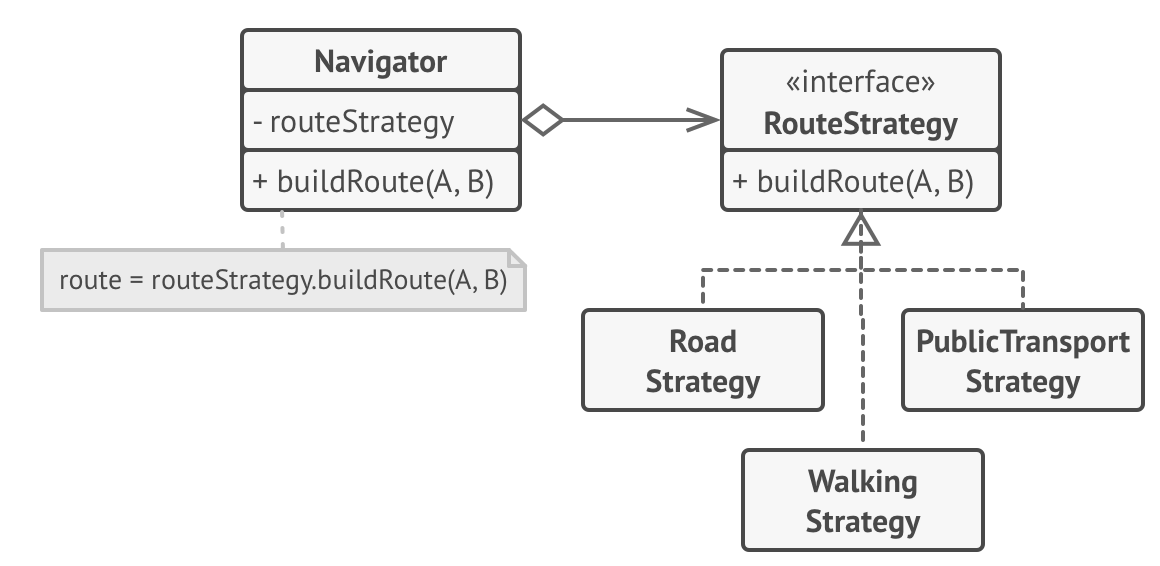
\includegraphics[width=\columnwidth]{../images/strategy.png}
                \caption{Strategy pattern \cite{StraPattern}}
            \end{figure}
        \end{column}
    \end{columns}

    
\end{frame}